    %\subsection{Description générale}
        %\subsubsection{Activités de l'entreprise et historique}
            %\paragraph{}
            %Quelques chiffres

            %\paragraph{}

        %\subsubsection{localisation}
            %\paragraph{}
            %Ses domaines d'activités.
            %\paragraph{}

        %\subsubsection{Organisation}
            %\paragraph{}
            %Ses domaines d'activités.
            %\paragraph{}

            %Son pôle de recherche.
            %\paragraph{}
            %Ses compétences, son marché.

\section{Sujet du stage}
Représenter le trafic aérien de la \textsc{Fir}\footnote{FIR: région d'information de vol, de l'anglais Flight Information Region) est une division de l'espace aérien permettant de faciliter le travail des organismes du contrôle aérien.} de Tahiti dans le logiciel Google Earth. Le logiciel GoogleEarth permet de représenter un espace tridimensionnel et de placer, à l’intérieur du logiciel, des indicateurs tels que des marqueurs de position, des lignes et des polygones. Le logiciel GoogleEarth utilise des fichiers externes de type \textsc{Xml}\footnote{\textsc{Xml}: Extensible Markup Language («langage extensible de balisage»), est un langage informatique de balisage générique.} pour tracer ou représenter ces graphismes. Le format de ces fichiers est ouvert et publié par Google. 

Il s’agit, à partir des traces fournies par le système de contrôle de Tahiti, d’afficher le trafic aérien circulant dans la \textsc{Fir} à des fins d’analyse, de vérification de trajectoire, de mesure de distance…

    
\section{Présentation de l’environnement}
    \subsection{\textsc{Dsna/Dti}}
La Direction des Services de la Navigation Aérienne est chargée de rendre le service de navigation aérienne pour l’État français. A ce titre, la \textsc{Dsna} est responsable de rendre les services de circulation aérienne, d’information aéronautique et d’alerte sur le territoire national et ceux d’outre-mer (\textsc{Dom, Tom , Pom}). La \textsc{Dsna} s’appuie sur deux directions pour exécuter cette mission:
\begin{itemize}
    \item La Direction des opérations ou \textsc{Do},
    \item la Direction de la Technique et de l’Innovation ou \textsc{Dti}.
\end{itemize}\medskip
La \textsc{Do} est l’acteur opérationnel du contrôle aérien tandis que la \textsc{Dti} est chargée du volet technique. Celui-ci consiste à réaliser ou acquérir les systèmes qui participent à l’exercice du contrôle aérien. Il s’agit de systèmes informatiques permettant d’assister le contrôleur dans ses activités, de chaînes radios pour communiquer avec les aéronefs, de systèmes de traitement de l’information météorologique…

La \textsc{Dti} réalise également de nombreuses études pour traiter les besoins des utilisateurs et les évolutions réglementaires. La \textsc{Dti} réalise le déploiement et le support opérationnel des systèmes qu’elle acquiert ou réalise. 

Enfin la \textsc{Dti} fait viser ses systèmes, procédures et formation par l’autorité de surveillance nationale (Direction de la Sécurité de l'Aviation Civile ou \textsc{Dsac}).

La DTI est structurée en domaines qui sont chacun en charge de plusieurs pôles de compétences :
\begin{itemize}
    \item Recherche et développement, R \& D
    \item Exigences opérationnelles des systèmes, \textsc{Eos}
    \item Gestion du trafic aérien, \textsc{Atm}
    \item Communication, navigation, surveillance, \textsc{Cns}
    \item Déploiement et Support Opérationnel, \textsc{Dso}
\end{itemize}\medskip

Chaque pôle couvre un ensemble de fonctions et d’expertises.

Pôle \textsc{Atm/Vig} :
\begin{itemize}
    \item Le pôle « Vol et information générale » (\textsc{Vig}) est responsable de la maîtrise d’ouvrages systèmes de traitements des plans de vol et informations générales, à ce titre, le pôle assure le suivi industriel de leur réalisation ou de leur acquisition. Le pôle \textsc{Vig} est également chargé de leurs maintiens en condition opérationnelles lorsqu’ils sont déployés.
    \item Le pôle \textsc{Atm/Vig} est notamment responsable de la maîtrise d’ouvrages de systèmes déployés en outre-mer. L’aéroport de Tahiti (Polynésie française) a récemment été modernisé avec un système entièrement acquis auprès d’un industriel, couplé à un radar dans le cadre du projet \textsc{Tiare}, qui s’est terminé en 2009.
\end{itemize}\medskip


\section{Le site de Tahiti}
    \subsection{Objectif contrôle aérien}
Le contrôle aérien est un ensemble de services \nref{servicesaerien} rendus par les contrôleurs aériens aux aéronefs afin d'aider à l'exécution sûre, rapide et efficace des vols. Les services rendus sont au nombre de trois, appelés « services de la navigation aérienne », dans les buts de:
\begin{itemize}
    \item prévenir les collisions entre les aéronefs et le sol ou les véhicules d'une part, et les collisions en vol entre aéronefs d'autre part (autrefois appelés « abordages »). Il consiste aussi à accélérer et ordonner la circulation aérienne,
    \item de fournir les avis et renseignements utiles à l'exécution sûre et efficace du vol : informations météorologiques, information sur l'état des moyens au sol de navigation, information sur le trafic (quand le service de contrôle n'est pas assuré dans cette zone),
    \item de fournir un service d'alerte pour prévenir les organismes appropriés lorsque les aéronefs ont besoin de l'aide des organismes de secours et de sauvetage, et de prêter à ces organismes le concours nécessaire.
\end{itemize}\medskip

    \subsection{Les services de la circulation aérienne\label{servicesaerien}}
Comme nous l'avons vu plus haut, le contrôle aérien rend plusieurs services. Nous allons voir ces services plus en détails.

        \subsubsection{Le service de contrôle}
Le service de contrôle est assuré dans les buts suivants:
\begin{itemize}
    \item Prévenir les collisions entre aéronefs ou entre un aéronef et un obstacle
    \item Accélérer et ordonner la circulation aérienne
\end{itemize}\medskip

Le plus important reste donc la sécurité des vols. Le contrôleur s'assure que rien n'arrivera à l'aéronef pendant son vol par des causes extérieures (autre avion, obstacle), et qu'il arrivera à sa destination le plus vite possible. En outre le contrôleur est responsable de la sécurité des vols sous sa juridiction.

Les moyens qu'utilise le contrôleur pour prévenir les abordages sont la séparation (anciennement l'espacement) et l'information de trafic.
\begin{itemize}
    \item La séparation consiste à ménager entre deux aéronefs une distance minimale, garantissant la sécurité de ces deux avions.
    \item L'information de trafic est une information précise sur la position d'un autre aéronef pouvant se rapprocher dangereusement. Le pilote peut ne pas voir qu'un avion se rapproche, l'information de trafic l'aide à voir, afin de permettre au pilote d'éviter l'aéronef conflictuel.
\end{itemize}\medskip

        \subsubsection{Le service d'information}
Le service d'information de vol est assuré sur tout le territoire français. En espace aérien contrôlé, il est assuré par le service de contrôle. Dans les espaces aériens non contrôlés, il est assuré par un organisme UIV (dans les CRNA) et SIV (dans les approches) en vol, ou AFIS sur un aérodrome.
Il consiste à délivrer aux aéronefs les renseignements et avis nécessaires à l'exécution sûre et efficace du vol. Ces renseignements peuvent être (liste non exhaustive) :
\begin{itemize}
\item Météorologiques : conditions météo sur un terrain, présences d'orages…
\item Information sur le trafic (à ne pas confondre avec l'information de trafic) : information sur un trafic connu ou inconnu, en fonction des éléments disponibles, pouvant interférer avec un aéronef.
\item État des aides à la navigation
\item État des équipements sol d'un terrain
\item Amendements de plan de vol
\item Information sur la position, aide aux pilotes perdus
\item Autres ...
\end{itemize}\medskip

        \subsubsection{Le service d'alerte}
Le service d'alerte est aussi vaste que naturel. Il consiste à répondre à tous les besoins des avions qui se disent en détresse, ou dont on peut penser qu'ils sont en détresse. Ce service recouvre des domaines très variés :
\begin{itemize}
\item Si un avion a déposé un plan de vol, et que le contrôle à l'arrivée a reçu confirmation qu'il a bien décollé, il doit surveiller que l'avion arrive bien à destination aux alentours de l'heure prévue, et lancer des recherches si ce n'est pas le cas.
\item Si un avion ne répond plus à la radio et disparaît du radar, le contrôleur doit vérifier si l'aéronef a eu un problème et s'il s'est écrasé ou posé en urgence. Il déclenche alors les secours pour rechercher l'épave et secourir les occupants.
\item Si un aéronef s'écrase sur la piste ou à proximité de l'aérodrome, il déclenche immédiatement les secours et coordonne leur action jusqu'à l'arrivée des renforts.
\item Si un pilote signale avoir des problèmes avec son aéronef de nature à entraver le bon déroulement du vol, le contrôleur peut lui donner une priorité absolue à l'atterrissage en écartant tous les autres aéronefs.
\item Si le contrôleur sait ou soupçonne qu'un aéronef est détourné, il prévient les autorités compétentes et leur apporte tout le secours nécessaire.
\end{itemize}\medskip

D'une manière générale, ce service est une autorisation légale à porter secours par tous les moyens à un pilote en difficulté. Tout être humain le ferait, mais le service d'alerte donne au contrôleur une justification légale pour retarder ou dérouter certains aéronefs afin de porter secours à un autre.

    \subsection{La zone de contrôle de Tahiti: \textsc{Fir}}
        \subsubsection{Le transport aérien}
L’île de Tahiti est desservie par l'Aéroport International Tahiti Faa'a, situé à 5km au Sud-Ouest de Papeete. Inauguré en 1961, et détenu à 57\% par le Territoire de la Polynésie Française10, c’est le plus important aéroport de la Polynésie française, et le seul aéroport international du territoire. Il s’agit donc de l’unique point d’entrée pour l’immense majorité des visiteurs mais également pour les habitants des autres îles de la Polynésie française.

L’aéroport assure les liaisons avec une dizaine de destinations internationales : Los Angeles, Paris, Auckland, Sydney, Tokyo, Rarotonga, Santiago, l’Île de Pâques, Noumea et Honolulu10. Conscient de l’importance des liaisons aériennes internationales dans le développement économique de l’île et du pays, le gouvernement a inauguré en 1998 sa propre compagnie aérienne : Air Tahiti Nui (ATN), qui dessert aujourd’hui 5 destinations à partir de Tahiti : Paris, Los Angeles, Tokyo, Auckland, Sydney.

Concernant le réseau domestique, l’aéroport dessert l’ensemble des archipels de la Polynésie. Air Tahiti est la seule compagnie à desservir régulièrement les îles polynésiennes, assurant la liaison avec une quarantaine d’îles et d’atolls. L’île de Moorea, située à 7 minutes de vol de Tahiti est desservie par Air Moorea, une filiale de la compagnie domestique d’Air Tahiti. L’aéroport de Tahiti est la plaque tournante du trafic aérien, puisque la majorité des destinations sont uniquement desservies par l’aéroport de Tahiti. La centralisation du réseau aérien accentue donc l’attraction et l’influence de Tahiti et de l’agglomération de Papeete sur le reste des îles polynésiennes.

        \subsubsection{Etendue de la \textsc{FIR}\label{Fir}}
\begin{figure}[!h]
\center
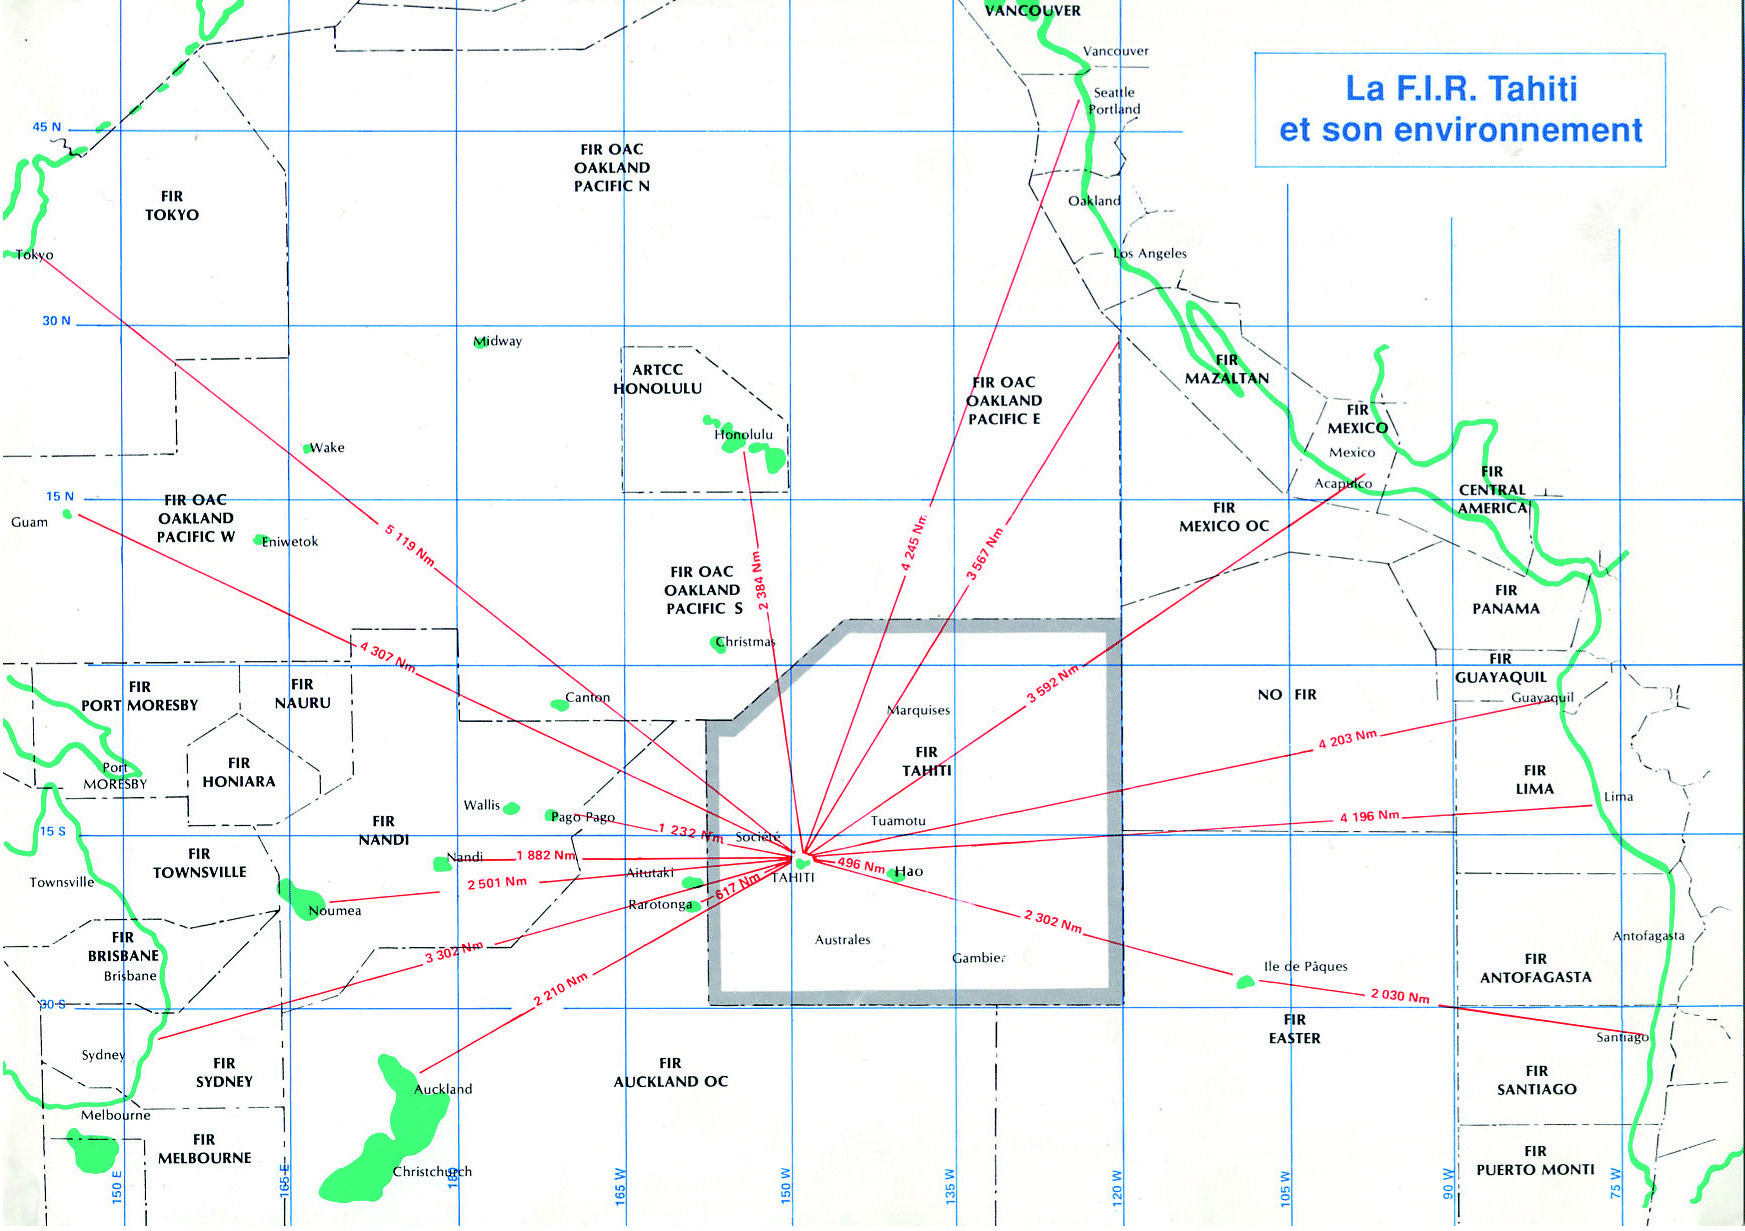
\includegraphics[width=15cm]{images/fir.png}
\caption{\textsc{Fir} de Tahiti dans la région Pacifique-Sud.}
\label{stats}
\end{figure}
La région d'information de vol de Tahiti ou « Flight Information Region » (\textsc{Fir} Tahiti) s'étend bien au-delà des eaux territoriales et déborde même sur l'hémisphère nord pour atteindre le parallèle 03\degre30' Nord, soit près de 3700 km de nord au sud et à peu près autant d'est en ouest, couvrant environ 12,5 millions de km$^2$.

Cette \textsc{Fir} constitue le volume au sein duquel la fourniture des services de la circulation aérienne sont assurés sous la responsabilité de l'administration française. Ces services comprennent :
\begin{itemize}
    \item alerte et sauvetage
    \item information de vol
    \item contrôle de la circulation aérienne
\end{itemize}\medskip
La FIR Tahiti est fréquentée par différents types de trafic :
\begin{itemize}
    \item les vols transpacifiques (entre la côte ouest des Etats-Unis et la Nouvelle-Zélande ou l'Australie)
    \item la desserte internationale de Tahiti (depuis et vers les Etats-Unis, la Nouvelle-Zélande, l'Australie, le Japon et le Chili)
    \item les vols intérieurs (desserte domestique des 47 aérodromes de Polynésie Française)
\end{itemize}\medskip

Plus de 40 contrôleurs aériens travaillent 24h/24 et 7j/7 dans la tour de contrôle de Tahiti-Faa'a.

Plus de 20 contrôleurs travaillent sur les aérodromes contrôlés des îles.

En 2006, le centre de contrôle a contrôlé 102 132 mouvements (+2,5\%), dont 71477 mouvements \textsc{Ifr}\footnote{\textsc{Ifr}: (soit, en anglais, Instrument flight rules) règles de vols aux instruments} et 30655 mouvements \textsc{Vfr}\footnote{\textsc{Vfr}: Visual flight rules, nom anglais de « Vol à vue »}.

        \subsubsection{La zone \textsc{Aci}:\label{Aci}}
Une fonction de contrôle spécifique, nommée \textsc{Aci}\footnote{\textsc{Aci}: Area Common Interest, soit une zone d'intérêts commun} ou zone \textsc{Aci}, a été développée dans le système \textsc{Eurocat-X} pour répondre à des besoins de contrôle. Il s’agit d’une zone particulière limitrophe à la \textsc{Fir} \nref{Fir} de Tahiti, dont la limite se situe à 50 miles nautiques de la \textsc{Fir}. La zone \textsc{Aci} encercle la \textsc{Fir}. Il est à noter que cette zone n’est pas sous la responsabilité des contrôleurs aériens français, cependant, les vols pénétrant dans cette région sont visualisés par le système Eurocat-X 

Ainsi en visualisant le trafic aérien dans la zone \textsc{Aci}, les contrôleurs peuvent maintenir les séparations entre les aéronefs. C'est-à-dire vérifier que les vols qui sont à l’extérieur et longent la \textsc{Fir} de Tahiti sont séparés des vols évoluant dans cette \textsc{Fir}.

    \subsection{Le système de contrôle: \textsc{Tiare}}
\textsc{Tiare} est le nom donné au projet qui a débuté en 2007 pour s'achever fin 2010. Ce projet visait à moderniser les moyens informatiques de contrôle du centre de Tahiti, de remplacer les systèmes vieillissants de visualisation du trafic (\textsc{Vivo}) et de gestion de plans de vol et d'informations générales (\textsc{Sigma}). La \textsc{Dti} a fait l'acquisition de deux systèmes différents pour couvrir l’ensemble des missions dévolue aux personnels du bureau de piste et du contrôle aérien.

Les situations de contrôle auxquelles doivent face les contrôleurs sont multiples, il y en a en effet à traiter les spécificités du contrôle océanique, du contrôle d’approche et inter-îles. Le système \textsc{Tiare} est construit à partir de plusieurs « produits sur étagère » :
\begin{itemize}
  \item \textsc{Eurocat-X}, système en charge du traitement radar et de la gestion plans de vols.
  \item \textsc{Atalis}, système en charge de la préparation des vols, de la gestion des \textsc{Notam}, et de la présentation d’informations générales au contrôleur tour et approche.
\end{itemize}\medskip

Les systèmes \textsc{Eurocat-X} et \textsc{Atalis} sont connectés au commutateur \textsc{Cagou}, raccordé aux liaisons externes (\textsc{Rsfta}). \textsc{Atalis} reçoit également des informations météorologiques en provenance du système local d’acquisition de ces données appelé \textsc{Caobs}. \textsc{Eurocat-X} est raccordé au radar secondaire du mont Marau et au réseau \textsc{Acars}.

%PREVOIR SHEMA

La zone Aci \nref{Aci}, a été développée spécifiquement dans le système \textsc{Eurocat-X} pour répondre à des besoins de contrôle.


    \subsection{L'\textsc{Ads-C}}

Avec l'\textsc{Ads-C} (Automatic Dependant Surveillance - Contract), l'avion utilise ses systèmes de navigation satellitaires ou inertiels pour automatiquement déterminer et transmettre au centre responsable sa position et d'autres informations.

Les informations transmises via l'\textsc{Ads-C} peuvent être:
\begin{itemize}
\item La position de l'avion,
\item Sa route prévue,
\item Sa vitesse (sol ou air),
\item Des données météorologiques (direction et vitesse du vent, température...).
\item Les informations de l'\textsc{Ads-C} sont transmises via des communications point à point, par \textsc{Vhf} ou par satellite. Les systèmes sol et embarqués négocient les conditions suivant lesquelles ces transmissions s'effectuent (périodiques, sur événement, à la demande, ou sur urgence).
\end{itemize}\medskip

L'\textsc{Ads-C} est typiquement utilisé dans les zones désertiques ou océaniques où il n'y a pas de couverture radar.

Les avantages de l'\textsc{Ads-C} sont :
\begin{itemize}
\item L'utilisation pour la surveillance des zones sans couverture radar.
\item La transmission de l'information "route prévue".
\item La liaison de données air/sol (comme pour le Mode S et l'\textsc{Ads-B}).
\end{itemize}\medskip

L'inconvénient de l'\textsc{Ads-C} est qu'il dépend entièrement de l'avion et de la correction des données qu'il transmet.




